\documentclass[graphics]{beamer}

\usepackage{graphicx}
\usepackage{verbatim}
\usepackage{wrapfig}
\useoutertheme{shadow}
%\usecolortheme{orchid}
\usecolortheme{seahorse}


% math commands
\newcommand{\be}{\begin{eqnarray}}
\newcommand{\ee}{\end{eqnarray}}
\newcommand{\beq}{\begin{equation}}
\newcommand{\eeq}{\end{equation}}
\def\simless{\mathbin{\lower 3pt\hbox
      {$\rlap{\raise 5pt\hbox{$\char'074$}}\mathchar"7218$}}}
\def\simgreat{\mathbin{\lower 3pt\hbox
      {$\rlap{\raise 5pt\hbox{$\char'076$}}\mathchar"7218$}}} %> or of order

% variables

\def\toonscale{0.45}
\def\mboxy#1{\mbox{\small #1}}


\begin{comment}
\AtBeginSection[]{
  \frame{
    \frametitle{Outline}
    \tableofcontents[currentsection]
  }
}
\end{comment}

\title{21cm intensity mapping: current results and future potential
}
%\subtitle{interim update}
\author[U. Pen]{Ue-Li Pen, Toronto
\\[8mm] 
}
\date{June 29, 2016}


\begin{document}

%\section*{Introduction}
\section{Current results}

\begin{comment}
  \subsection{Outline}

  \frame{
    \frametitle{Outline}
    \tableofcontents
  }
\end{comment}

\frame{\maketitle}



  \frame{
\vspace{-0.5in}
    \frametitle{History}
    \begin{itemize}
        \item Intensity mapping: LSS using HI in galaxies without
          detecting individual galaxies
        \item Morales\&Wyithe ARAA, April 2010: {\it The impending EoR measurements will teach the observational community how to perform precision cosmological measurements at low radio frequencies. This experience will be invaluable for both subsequent EoR measurements and first generation intensity mapping machines.}
        \item Chang et al May 2010: first GBT-IM detection
        \item mushrooming of dedicated experiments: CHIME,
          CRT-Tianlai, HIRAX, 
%          \vspace{-0.15in}
    \end{itemize}
  }


  \frame{
\vspace{-0.5in}
    \frametitle{GBT-IM}
    \begin{itemize}
        \item 650 hours in 700-900 MHz band, $0.54<z<1$
        \item initial power spectrum: cross correlation with WiggleZ,
          auto spectrum
        \item measures $\Omega_{HI}br=0.43\pm 0.08$ (Masui et al 2013,
          Switzer et al 2013)
        \item archival discovery of FRB110523
%          \vspace{-0.15in}
    \end{itemize}
\vspace{-0.5in}\hspace{2.6in}
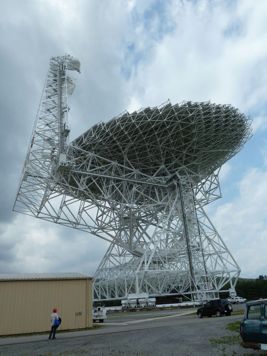
\includegraphics[width=1.5in]{Figures/gbt-eric.png} \vspace{-0.5in}
  }
  \frame{
\vspace{-0.2in}
    \frametitle{map}
\hspace{-0.2in}\includegraphics[width=4.5in]{Figures/sec_A_15hr_41-90_clean_map_I_RADec.mp4}
  }
  \frame{
\vspace{-0.2in}
    \frametitle{residual}
\hspace{-0.2in}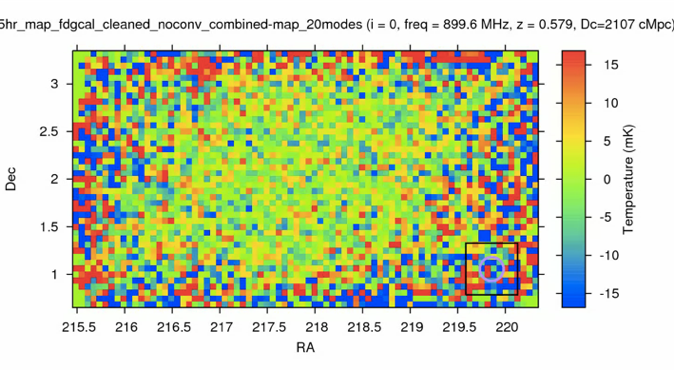
\includegraphics[width=4.5in]{Figures/gbt-residual.png}
  }
  \frame{
    \frametitle{power}
\vspace{-0.2in}
\hspace{-0.3in}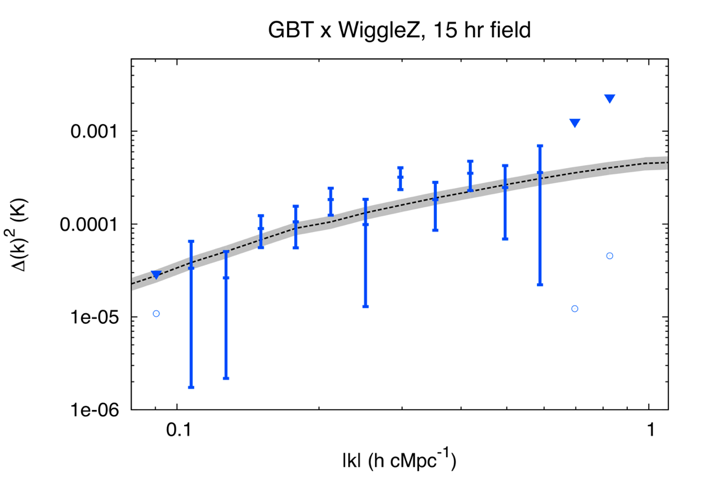
\includegraphics[width=4.5in]{Figures/gbt-power.png}
  }

  \frame{
\vspace{-0.5in}
    \frametitle{Parkes-IM}
    \begin{itemize}
      \item 500 beam-hours on 2dF field
      \item measure 21cm $z<0.2$ auto-power, cross-power, RSD, $\Omega_{HI}$
      \item analysis in progress
%          \vspace{-0.15in}
    \end{itemize}
%\vspace{-0.1in}
\hspace{.3in}
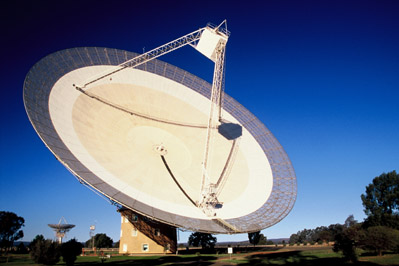
\includegraphics[width=3in]{Figures/parkes.jpg}\vspace{-0.4in}
  }

\section{Experiments under construction}
  \frame{
    \frametitle{CHIME}
    \begin{itemize}
        \item Pathfinder operating: sky maps
        \item Full CHIME mechanial construction completed, electronics
          in deployment, on air in 2017
    \end{itemize}
%\vspace{-0.1in}\hspace{.3in}
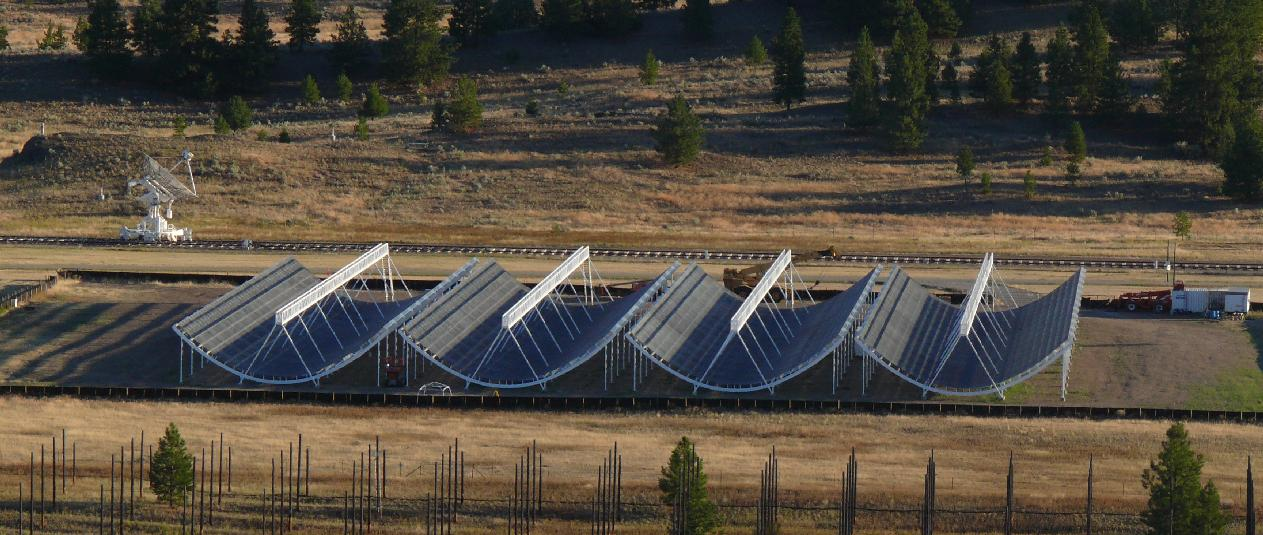
\includegraphics[width=4in]{Figures/Chime-medium.jpg}
}
  \frame{
\vspace{-0.2in}
    \frametitle{659 MHz - dirty}
\hspace{-0.2in}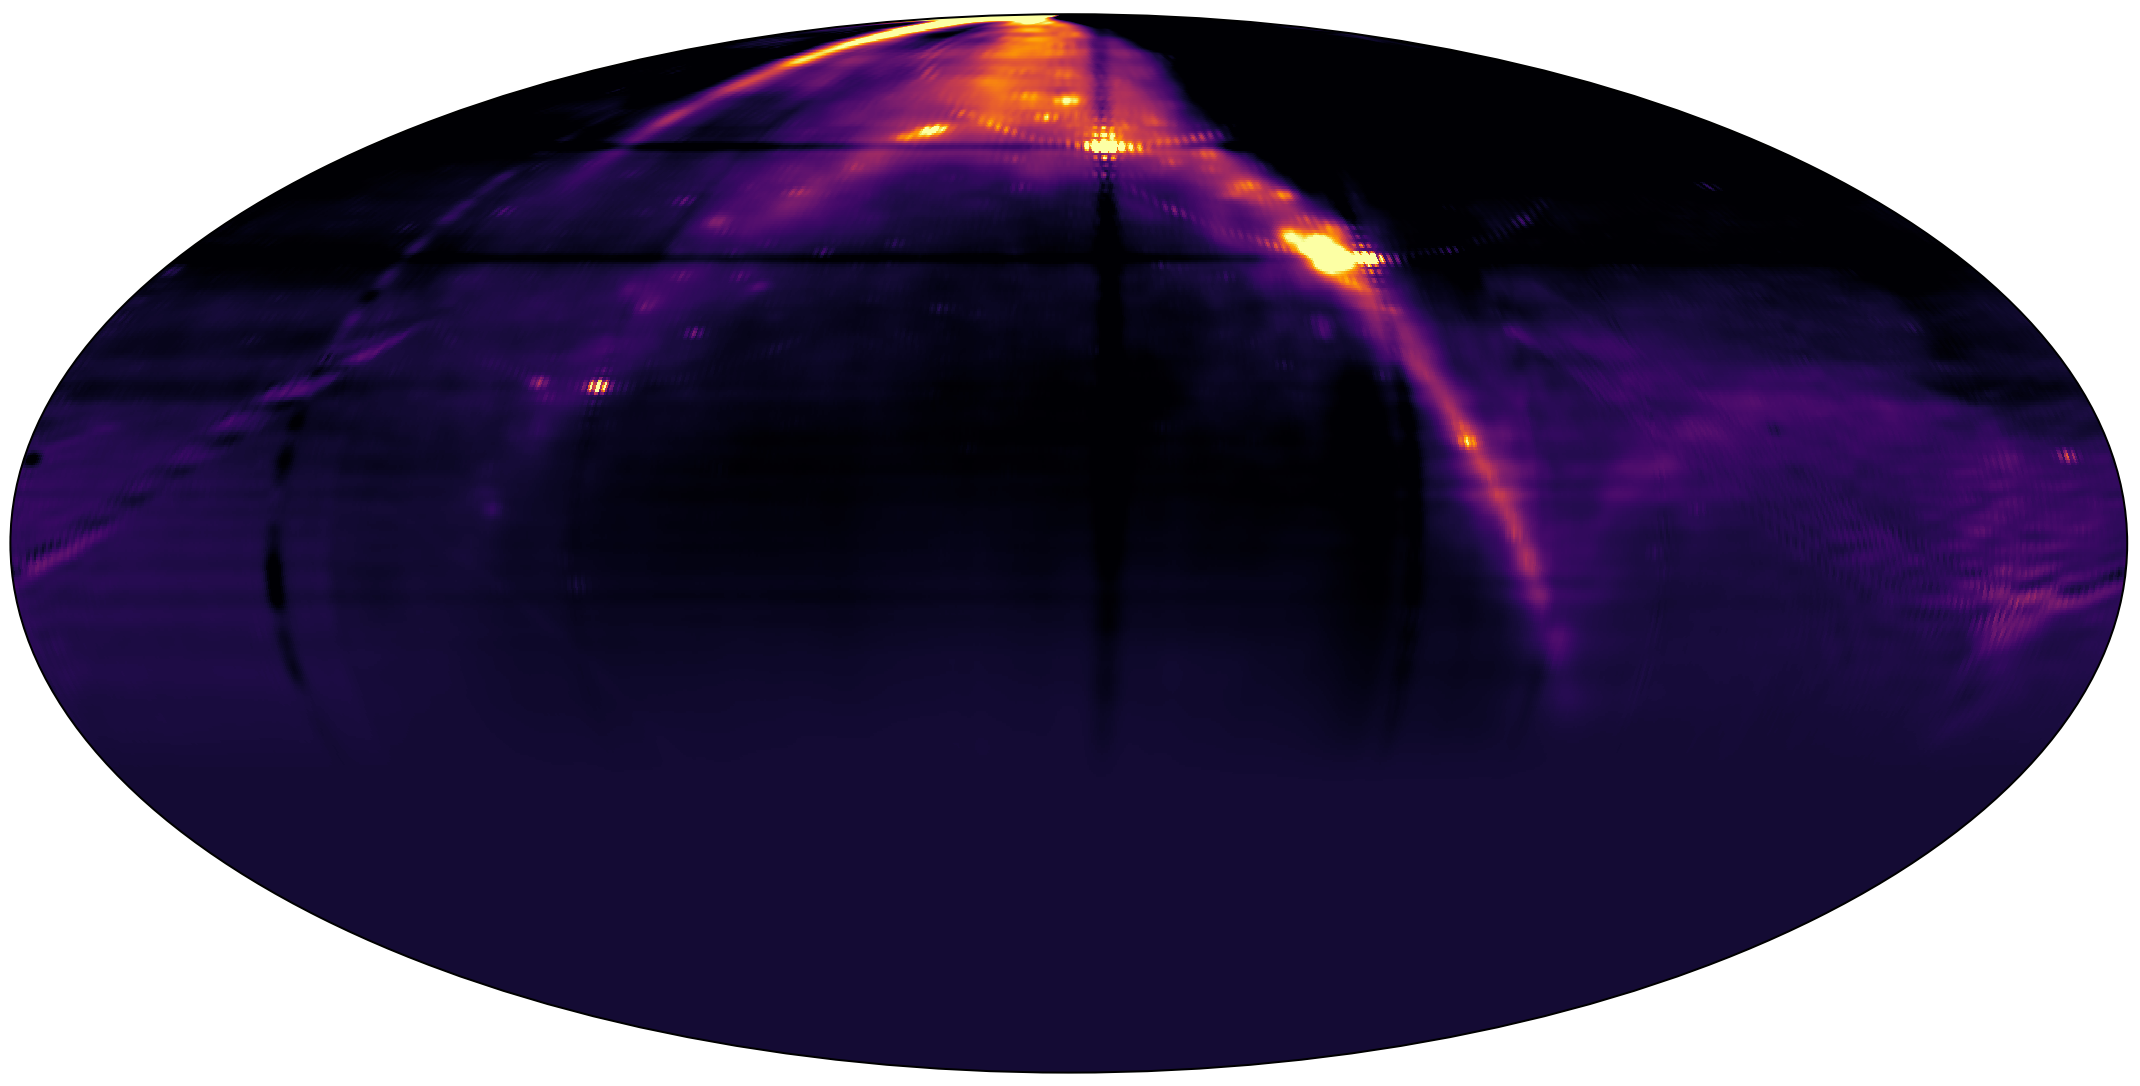
\includegraphics[width=4.5in]{Figures/chime-dirty.png}
  }
  \frame{
\vspace{-0.2in}
    \frametitle{Simulated Haslam - dirty}
\hspace{-0.2in}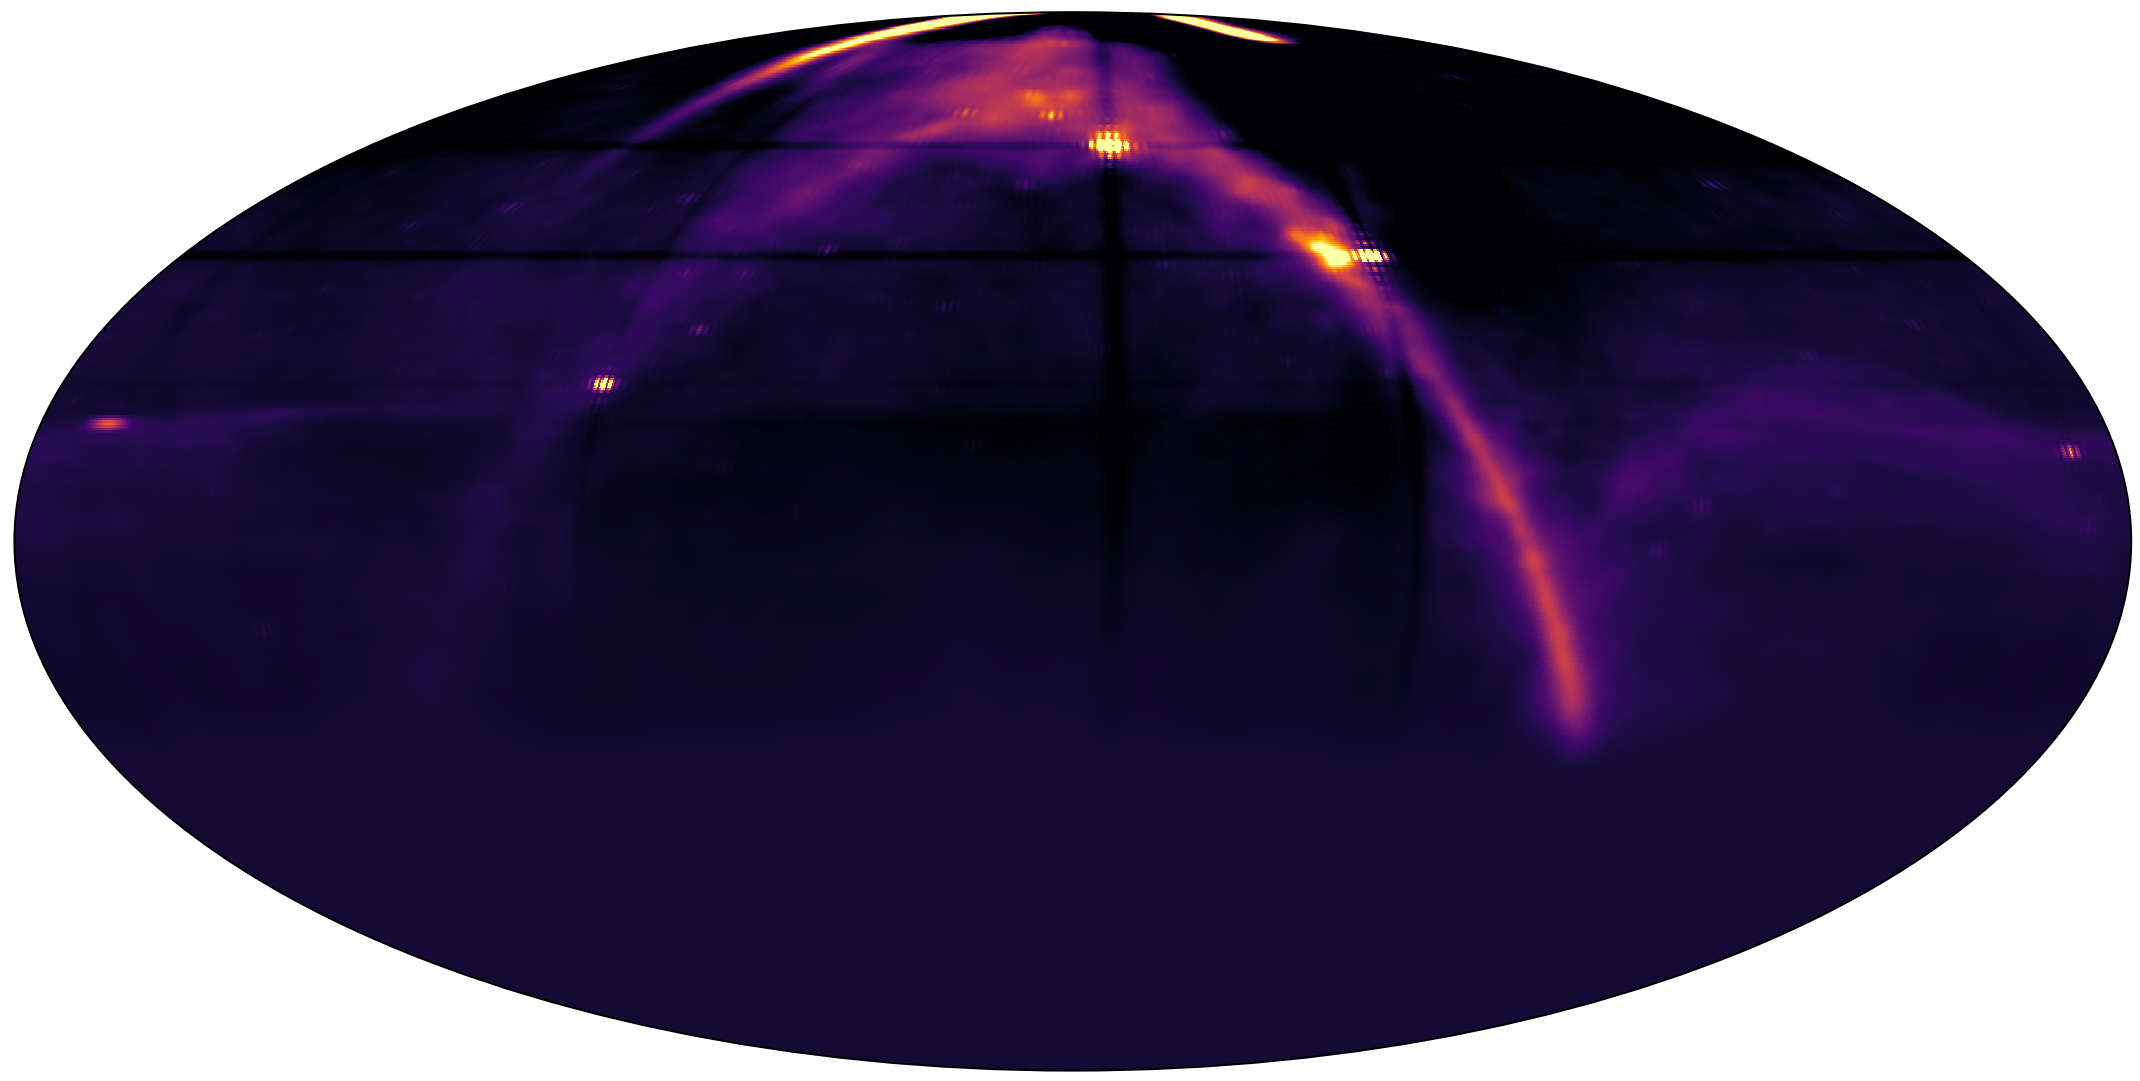
\includegraphics[width=4.5in]{Figures/chime-sim.png}
  }

  \frame{
    \frametitle{Tianlai}
    \begin{itemize}
        \item in Xinjiang, China
        \item currently commissioning
    \end{itemize}
%\vspace{-0.1in}\hspace{.3in}
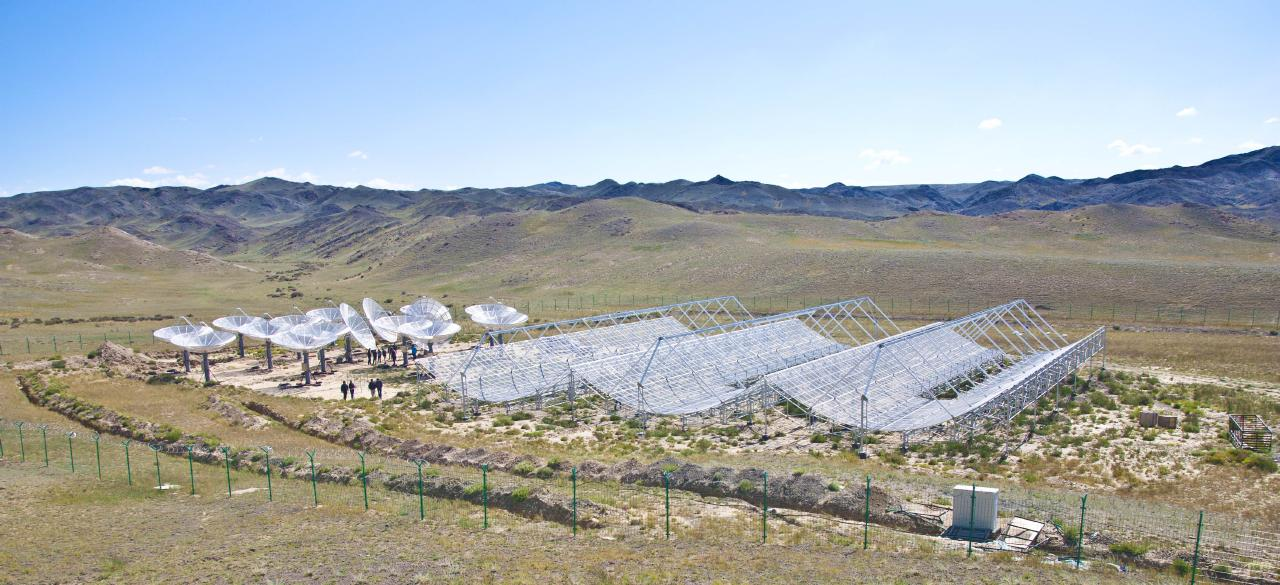
\includegraphics[width=4in]{Figures/tianlai-medium.jpg}
}

  \frame{
    \frametitle{HIRAX}
    \begin{itemize}
        \item Karoo, SA
        \item most ambitious IM-BAO project, doubles as pulsar and FRB engine
    \end{itemize}
%\vspace{-0.1in}\hspace{.3in}
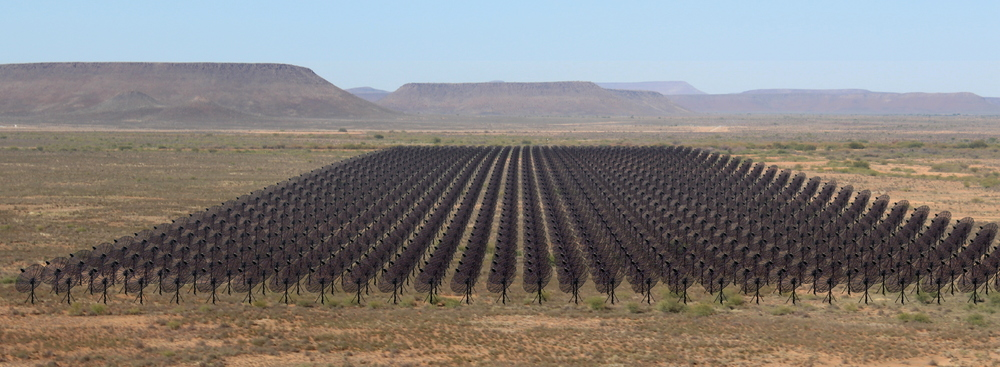
\includegraphics[width=4in]{Figures/hirax-karoo-s.jpg}
}
\section{Future Experiments}
  \frame{
    \frametitle{Proposed/Planned}
    \begin{itemize}
        \item BINGO, BAOBAB, Carpe, etc
        \item CO, L$_\alpha$, other lines
    \end{itemize}
}
\section{Lessons learned}
  \frame{
    \frametitle{Observing strategy}
    \begin{itemize}
        \item drift scan: all approaches now utilize drift scans
        \item $m$-mode transform: eliminate E-W mode mixing! (Shaw et
          al 2013)
        \item scale invariant N-S imaging: apodization to common beam
    \end{itemize}
}
  \frame{
    \frametitle{Filled aperture}
    \begin{itemize}
        \item no 'wedge' issues
        \item clean side lobes
        \item large mosaics
    \end{itemize}
}
  \frame{
    \frametitle{Outlook}
    \begin{itemize}
        \item 21cm signal-foreground sweetspots: $z<2,\ z \sim 8, z
          \sim 15$
        \item FAST aperture array, large low frequency cylinder
          arrays: FFT telescopes
    \end{itemize}
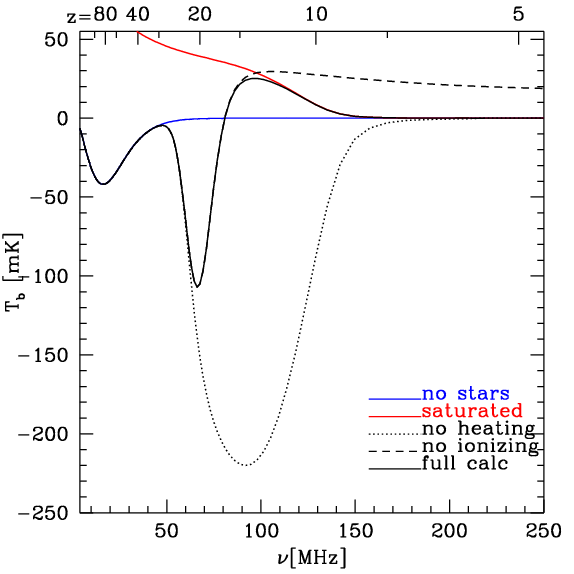
\includegraphics[width=1.9in]{Figures/pedplot-nu.png} Pritchard \&
Loeb 2010
}

\end{document}
